\documentclass[tikz,border=8pt]{standalone}
% Style commun des schémas : thème clair / sombre (couleurs des thèmes GitHub), fond transparent.
\usepackage[T1]{fontenc}
\usepackage{tgheros}
\renewcommand{\familydefault}{\sfdefault}
\usepackage{tikz}
\usetikzlibrary{positioning,arrows.meta,calc,fit,backgrounds}
\ifdefined\darktheme
  \definecolor{fg}{HTML}{E6EDF3}  \definecolor{muted}{HTML}{9198A1}
  \definecolor{line}{HTML}{8B949E} \definecolor{boxfill}{HTML}{151B23}
  \definecolor{boxline}{HTML}{3D444D}
  \definecolor{blue}{HTML}{4493F8} \definecolor{orange}{HTML}{DB6D28}
  \definecolor{green}{HTML}{3FB950} \definecolor{red}{HTML}{F85149}
  \definecolor{purple}{HTML}{AB7DF8}
\else
  \definecolor{fg}{HTML}{1F2328}  \definecolor{muted}{HTML}{59636E}
  \definecolor{line}{HTML}{59636E} \definecolor{boxfill}{HTML}{F6F8FA}
  \definecolor{boxline}{HTML}{D1D9E0}
  \definecolor{blue}{HTML}{0969DA} \definecolor{orange}{HTML}{BC4C00}
  \definecolor{green}{HTML}{1A7F37} \definecolor{red}{HTML}{CF222E}
  \definecolor{purple}{HTML}{8250DF}
\fi
\tikzset{
  every node/.style={text=fg, font=\small},
  block/.style={draw=boxline, fill=boxfill, rounded corners=3pt, line width=0.7pt,
                minimum height=11mm, minimum width=30mm, align=center, inner sep=5pt},
  sub/.style={font=\scriptsize, text=muted},
  wire/.style={line width=1pt, -{Stealth[length=2.6mm]}},
  biwire/.style={line width=1pt, {Stealth[length=2.6mm]}-{Stealth[length=2.6mm]}},
  lbl/.style={font=\scriptsize, text=muted, fill=none, inner sep=2pt},
}

\begin{document}
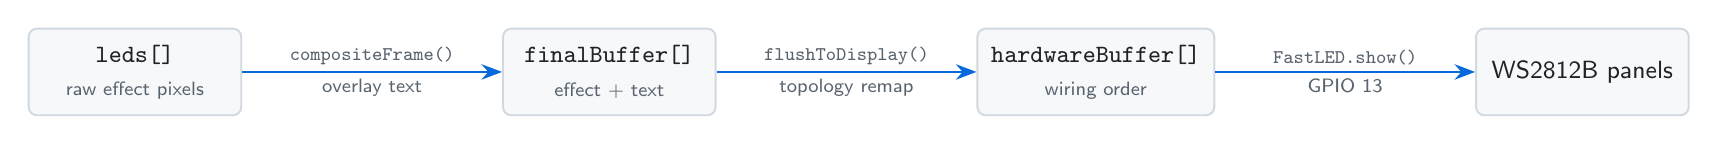
\begin{tikzpicture}[node distance=33mm]
  \node[block, minimum width=27mm] (a) {\texttt{leds[]}\\[1pt]\textcolor{muted}{\scriptsize raw effect pixels}};
  \node[block, minimum width=27mm, right=of a] (b) {\texttt{finalBuffer[]}\\[1pt]\textcolor{muted}{\scriptsize effect + text}};
  \node[block, minimum width=27mm, right=of b] (c) {\texttt{hardwareBuffer[]}\\[1pt]\textcolor{muted}{\scriptsize wiring order}};
  \node[block, minimum width=27mm, right=of c] (d) {WS2812B panels};
  \draw[wire, blue] (a) -- node[above, lbl]{\texttt{compositeFrame()}} node[below, lbl]{overlay text} (b);
  \draw[wire, blue] (b) -- node[above, lbl]{\texttt{flushToDisplay()}} node[below, lbl]{topology remap} (c);
  \draw[wire, blue] (c) -- node[above, lbl]{\texttt{FastLED.show()}} node[below, lbl]{GPIO 13} (d);
\end{tikzpicture}
\end{document}
